cd ~/%!TEX root = ../dokumentation.tex


\chapter{Implementation}\label{cha:Implementation}

\section{Lexer}\label{sec:ImplementationLexer}

As mentioned in chapter \ref{sec:ConceptLexer} the implementation of the lexer consists of the definition of tokens in form of regular expression. The following paragraph presents defined tokens and their regular expressions.

\subsubsection{Ignored symbols}
It is possible to declare certain symbol as symbol that should be ignored. However, if a symbol is declared as ignored but is specifically mentioned in another token, then if the sequence of characters represent that token, the ignored symbol is not ignored. 
In this project, tabs and white spaces are ignored as they don not have any special meaning other than providing clarity. 
Also, newlines are generally ignored because as can be seen below there are rules that cover multiple lines. If newlines wouldn't be ignored it would be difficult to ??

\begin{lstlisting}[basicstyle=\scriptsize	,caption= Example of a multi line production rule,label= lst:Lexer_example_multiline]
<annotated_formula>    ::= <thf_annotated> | <tff_annotated> | <tcf_annotated> |
                           <fof_annotated> | <cnf_annotated> | <tpi_annotated>
\end{lstlisting}

Apart from the ignored symbols, there are 13 defined tokens:

\subsubsection{Expressions}

Expressions can either grammar, token, strict or macro expression. REFERENCE
A non terminal symbol followed by the symbol itself (::=,:==,:::,...). The non terminal symbol and the symbol build a single token and are not identified as two tokens to avoid further ambiguity while parsing. Otherwise it would be difficult for the parer to determine whether the non terminal symbol that describes the rule is the start of a new rule or does still belong the previous rule because as mentioned the rules can cover multiple lines.

\textit{Regular expression of grammar expression:}  $'<\backslash w+>[\backslash s]*::='$

$\backslash w+$ matches any alphanumeric and underscore character that can occur more than one time.
$[\backslash s]*$ matches an arbitrary amount of white spaces.

\subsubsection{Non terminal symbol}

A non terminal symbol starts with \dq <\dq and ends with \dq >\dq. In between there is any arbitrary sequence of numbers, underscores and small or capital letters.

\subsubsection{Terminal symbol}

\subsubsection{Comment}

A comment is identified by the lexer as a start of a new line followed by a percentage sign followed by an arbitrary character and ends with a newline. Because the percentage sign is also part of the terminal symbols, it is necessary to check whether the percentage sign is in a newline because the terminal symbol is not because the percentage symbol when used as terminal symbol is embedded in square brackets.    

\subsubsection{Meta-Symbols}

Meta-Symbols include open and close parentheses \dq( )\dq, open and close square brackets \dq[ ]\dq, asterisks \dq *\dq and vertical bars \dq |\dq.

They are recognized by the symbol itself and have a greater meaning for the parser as they impact the to be build data structures. 

\subsubsection{Ambiguity}

The following example could either be matched as one comment token or as comment, grammar expression, non terminal symbol, terminal symbol, non terminal symbol.
This ambiguity is solved because by convention the lexer matches the longest possible token, the sequence of characters is matched as one comment.
\begin{lstlisting}[basicstyle=\scriptsize	,caption= Example of a commented out production rule,label= lst:Lexer_example]
%----   <formula_role> ::= <user_role>-<source>
\end{lstlisting}
\section{Parser}\label{sec:ImplementationParser}

The parser is taking the tokens from the lexer and matches them to defined production rules.




comment block reimplement equal operator

\subsection{Data Types}\label{sec:ImplementationDataTypes}
Figure \ref{fig:ImplementationUMLExpressions} contains the UML modelling of the data types described in section \ref{sec:ConceptParserDataStructure}.
\begin{figure}[H]
\centering
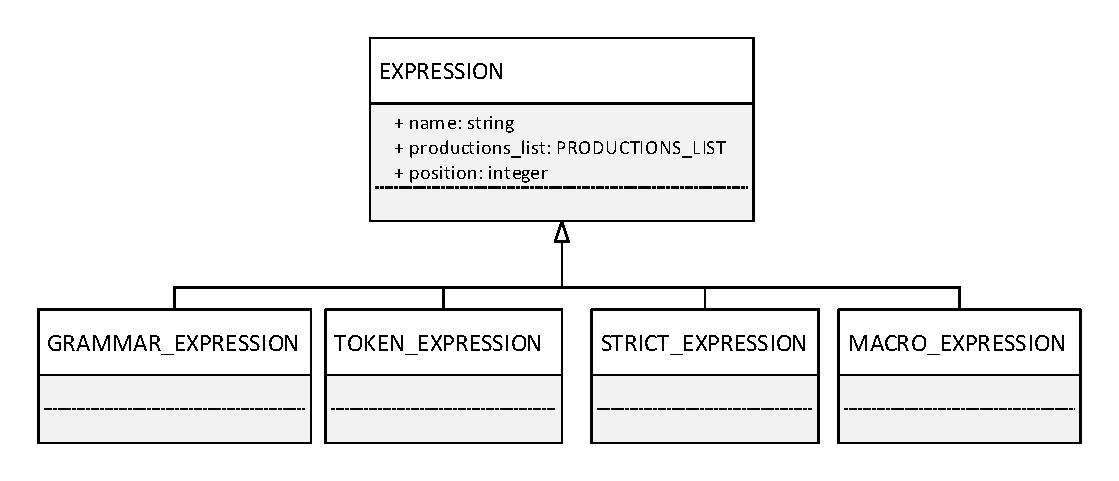
\includegraphics[width=1\textwidth]{images/uml_data_types_expressions.pdf}
\caption{UML diagram for expressions}
\label{fig:ImplementationUMLExpressions}
\end{figure}
\section{Graph Generation}\label{sec:ImplementationGraphGeneration}

\begin{algorithm}[H]
\caption{Graph Generation Algorithm}
\begin{algorithmic}[1] 
\Require node
%\ENSURE $y = x^n$
\State searchProductionsListForNT(node, node.productionslist)
\If {Node has children}
	\For{\texttt{Each child}}
		\State buildGraphRek(child)
	\EndFor
\EndIf
\end{algorithmic}
\end{algorithm}

\section{GUI}\label{sec:GUI}
\section{Console Interface}\label{sec:Console Interface}
-argparse Python offers a library for console interfaces.
-options for path to grammar and control file
-option for output path